\documentclass[a4paper, 11pt]{article}
\usepackage[text={17cm, 24cm}, top=3cm, left=2cm, includefoot]{geometry}
\usepackage{times}
\usepackage[hidelinks]{hyperref}
\usepackage{multirow}
\usepackage{multicol}
\usepackage{hyperref}

\usepackage{graphicx}
\usepackage{color}
\usepackage[slovak]{babel}

\usepackage{color}

\begin{document}
\begin{titlepage}
\begin{center}

\includegraphics[width=0.77\linewidth]{img/fitlogo1_cz.pdf} \\
\vspace{\stretch{0.382}}
\Huge
\textsc{\textbf{Dokumentácia projektu}} \\
\Large\textbf{Mikroprocesorové a vstavané systémy  \\Ovládanie RGB LED} \\
\vspace{\stretch{0.618}}
\LARGE

15.12.2022 
\hfill
\begin{tabular}{l l l}
   \textbf{Šimon Kadnár} & \textbf{xkadna00}  \\
\end{tabular}

\end{center}
\end{titlepage}

\section{Úvod}
Zadaním projektu bolo implementovať vstavanú aplikáciu na doske ESP32, ktorá bude schopná ovládať skupinu LED diod a jednu RGB led pomocou WIFI rozhrania. Výsledná aplikácia obsahuje niekoľko rôznych animácií svetiel a možnosť upraviť ich rýchlosť. Aplikácia bola implementovaná v jazyku C++ cez prostredie PlatromIO na platforme Arduino.

\section{Zapojenie hardware}
Pri riešení tohto projektu boli použité porty(GPIO): 2, 5, 13, 12, 14, 27.

\subsection{Využitie portov}
\begin{itemize}
    \item Port 2 - značí príjem požiadavku
    \item Port 5 - ovláda ľavú diódu
    \item Port 13 - nastavuje červenú farbu na RGB led
    \item Port 12 - nastavuje zelenú farbu na RGB led
    \item Port 14 - nastavuje modrú farbu na RGB led
    \item Port 27 - ovláda pravú diódu
\end{itemize}
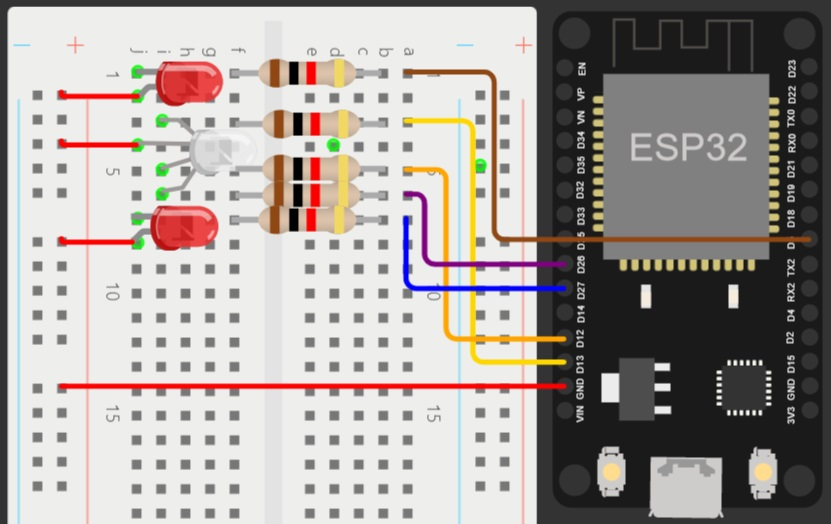
\includegraphics{img/zapojenie.jpg}

\section{Popis riešenia}
Na začiatku sa vo funkcii \textit{setup()} nastavia výstupné piny, vytvorí sa proces \textit{animation\_mod()}, ktorý ovláda výstupe piny pomocou volania funkcie pre konkrétnu animáciu. Následne sa vytvorí wifi sieť(rgb\_esp32) a založí sa server na ktorom sa nachádza ovládacia stránka. Potom nasleduje funkcia \textit{loop()} v ktorej ak je k dispozícií nový klient tak sa mu vygeneruje stránka s aktuálnym nastavením. V prípade, že dôjde k stlačeniu jedného z možných nastavení animácie funkcia obsahuje sadu podmienok ktorá detekuje zmenu url a podla toho buď zmení rýchlosť v premennej \textit{speed} (zavolaním funkcie \textit{get\_speed()}) alebo nastaví do premennej \textit{mod} hodnotu odpovedajúcej animácií a vynuluje riadiace premenné cnt1 a cnt2.

\subsection{Globálne premenné}
\begin{itemize}
    \item cnt1, cnt2 -- riadia priebeh animácie, 
    \item mod -- určuje typ animácie,
    \item speed -- určuje rýchlosť animácie
    \item header -- obsahuje odoslané informácie od klienta
\end{itemize}

\subsection{knižnice}
\begin{itemize}
    \item  stdio.h - práca so stringami
    \item  WiFi.h -- slúži pre vytvorenie vlasntej wifi a vytvorenie servera
    \item  ESPmDNS.h -- slúži pre prekrite ip adresy nazvom
\end{itemize}

\subsection{animation\_mod()}
Na začiatku sa nachádza nekonečný cyklus v ktorom sa nachádza sada podmienok kde sa najskôr určí, ktorá animácia má byť spustená podľa premennej \textit{mod}. Následne sa volá funkcia s danou animáciou (funckie: \textit{animation1()}, \textit{animation2()},...). Každá z nich obsahuje sadu podmienok, ktoré riadia priebeh animácie pomocou premenných \textit{cnt}, \textit{cnt1} a \textit{cnt2}, podľa ich inkrementácie. Na konci sa nachádza časovač ktorý obsahuje hodnotu \textit{speed} podľa ktorej sa určuje akou rýchlosťou má bežať vybraná animácia.

\subsection{get\_speed()}
Funkcia pracuje s premenou \textit{header}, ktorú prejde v cykle a nájde požadovanú rýchlosť, ktorú uloží do premennej \textit{speed}, čím dôjde k zmene rýchlosti vybranej animácie.

\section{Ovládanie}
Po spustení aplikácie je potrebné sa pripojiť na wifi sieť \textit{rgb\_esp32}, ktorú vysiela zariadenie. Následne je potrebné sa pripojiť na ovládaciu stránku cez preferovaný prehliadač zadaním \href{http://192.168.4.1}{http://192.168.4.1} alebo \href{http://esp32}{http://esp32}. Po pripojení na stránku sa zobrazí jedno tlačítko \textit{OFF} ktoré po stlačení sprístupní ďalšie 4 tlačítka ktoré ovládajú typ animácie a jedno textové pole do ktorého je možné zadať ľubovoľnú rýchlosť vybranej animácie. Po stlačení tlačidla sa na doske rozsvieti na malú chvíľu, červené svetlo, ktoré signalizuje prijatie požiadavku zo siete. V prípade, že chceme vypnúť animácie stačí stlačiť spodné tlačítko \textit{ON}. \\ \\
Demonštračné video:
\href{https://drive.google.com/file/d/1CSQYQpGuNmzeRpa_-Hc1tSbUmXrdMQXM/view?usp=share_link}{\color{blue}{Demo}}



\begin{figure}
     \centering
    \scalebox{0.25}{
\includegraphics{img/stranka2.jpg}}\hspace{-0.075cm}
    \scalebox{0.25}{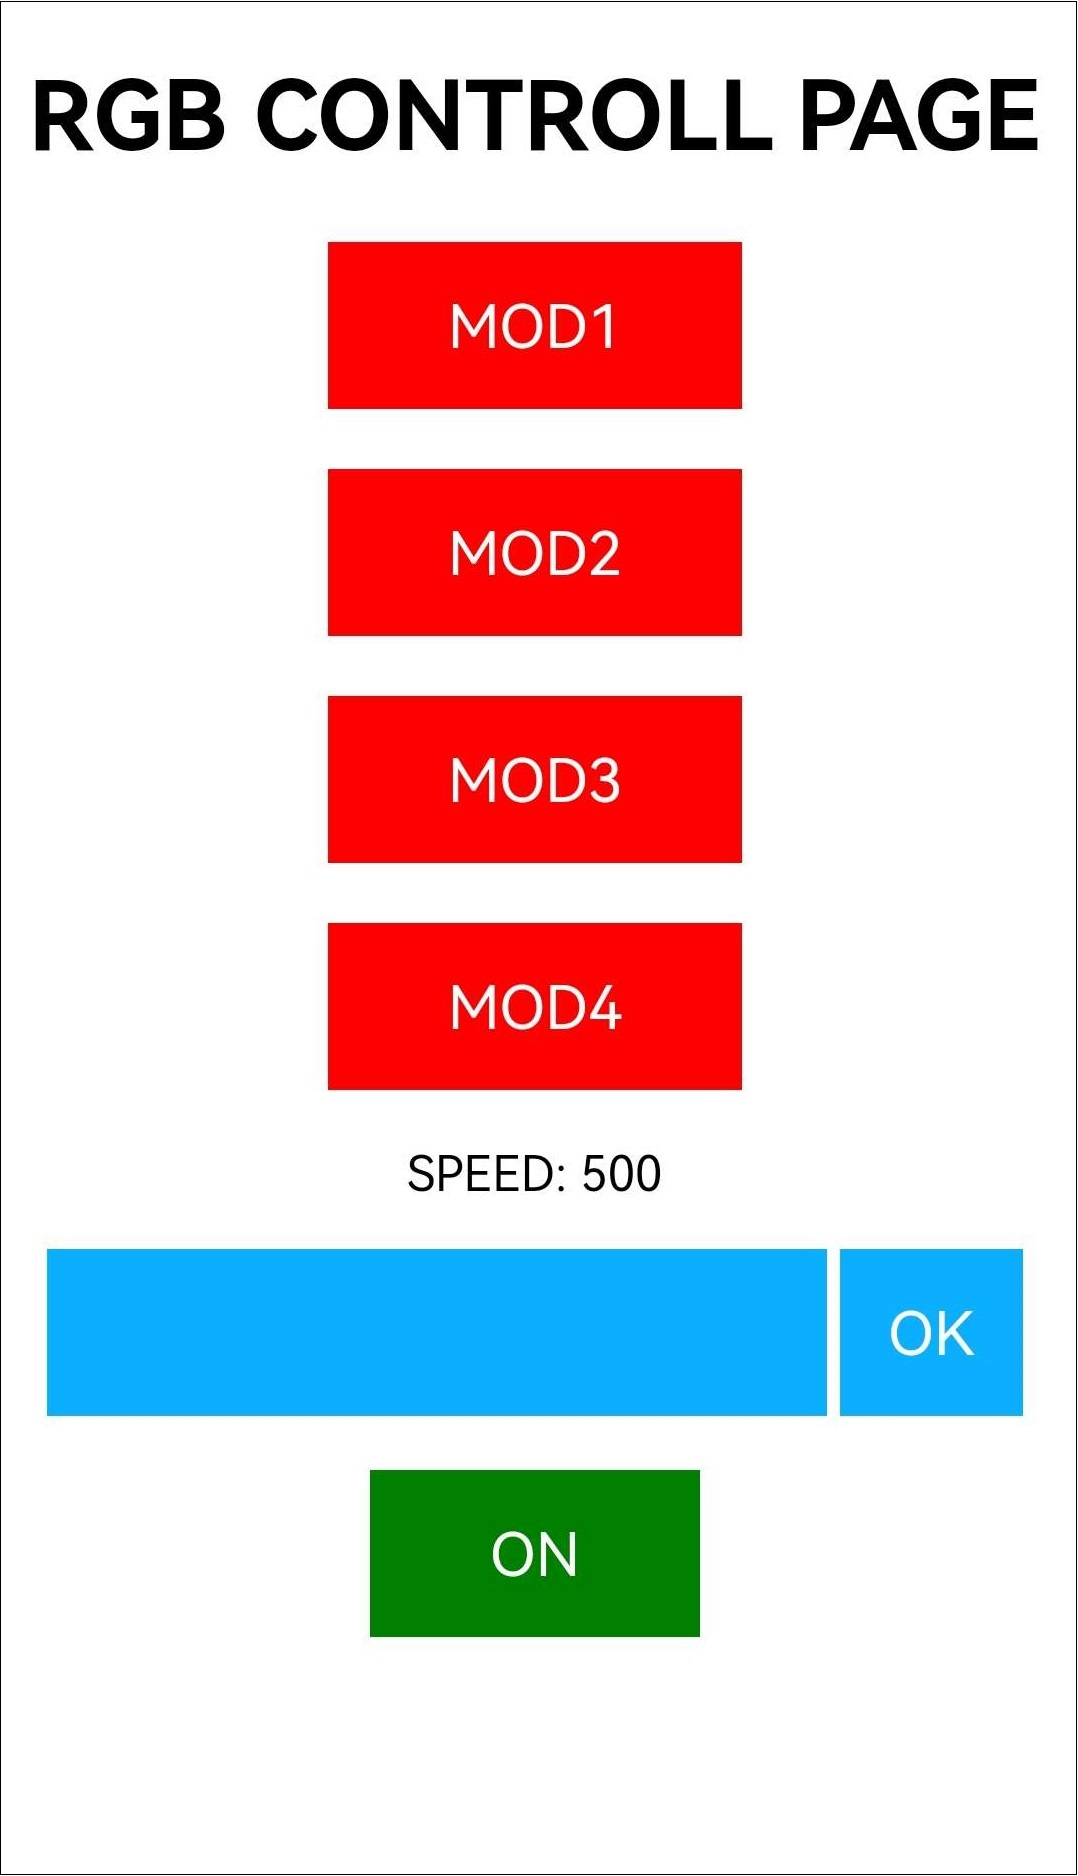
\includegraphics{{img/stranka1.jpg}}}
     \label{fig:my_label}
 \end{figure}



\section{Záver}
Výsledná aplikácia obsahuje 4 tlačidlá slúžiace pre nastavenie typu animácie, 1 textové pole pre zadávanie ľubovoľnej rýchlosti a jedno tlačidlo pre vypnutie animácie. Možné problémy sú s prekrytím ip adresy pomocou protokolu mDNS, ktorá nefunguje na niektorých mobilných zariadeniach a je teda zapotreby sa pripojiť na ovládaciu stránku pomocou ip adresy.

\subsection{Hodnotiaci kľúč}
E = 1\\
F = 4,5\\
Q = 2\\
P = 1\\
D = 4\\
(0,25 + 0,75 · F/5) · (E + F + Q + P + D) = 11,5

\section{Literatura}
\href{https://randomnerdtutorials.com/esp32-web-server-arduino-ide/
}{https://randomnerdtutorials.com/esp32-web-server-arduino-ide/}
\end{document}